% !TEX root = ../termpaper.tex
% first example section
% @author Thomas Lehmann
%

\section{Einleitung}
Das Ziel dieser Arbeit ist es, die Korrelation zwischen den Ergebnissen eines Random Walks und verschiedenen Zentralitätsmaßen in Netzwerken zu untersuchen. Zentralität ist ein fundamentales Konzept in der Netzwerkforschung, das misst, wie wichtig oder einflussreich ein Knoten in einem Netzwerk ist. Es gibt verschiedene Arten von Zentralitätsmaßen, die unterschiedliche Aspekte der Wichtigkeit eines Knotens erfassen. In dieser Arbeit werden die drei wichtigsten Zentralitätsmaße betrachtet: Gradzentralität (Degree centrality), die angibt, wie viele direkte Verbindungen ein Knoten zu anderen Knoten hat; Closeness-Zentralität (Closeness centrality), die misst, wie schnell ein Knoten von anderen Knoten im Netzwerk erreicht werden kann; und Betweenness-Zentralität (Betweenness centrality), die angibt, wie oft ein Knoten auf den kürzesten Wegen zwischen anderen Knoten liegt. Diese Maße sind entscheidend, um zu verstehen, wie Information oder Einfluss in einem Netzwerk fließt und welche Knoten als „Brücken“ oder besonders einflussreich gelten. 

Dabei werden zufällig generierte Graphen auf Basis des Erdős-Rényi Modells verwendet, bei dem die Anzahl der Knoten (n) und die Kantenwahrscheinlichkeit (p) variieren. Ziel ist es, zu analysieren, wie diese Parameter die Struktur des Netzwerks beeinflussen und wie sie die Korrelation zwischen den Zentralitätsmaßen und den Random Walk Ergebnissen verändern. Am Ende des Experiments wird auch die Frage aufgeworfen, ob die „relative Besuchszahl eines Random Walks näherungsweise proportional zum Knotengrad“ eines Netzwerkknotens sein könnte. 

\section{Ansatz und Vorüberlegungen}
\subsection{Zentralität und Zusammenhängigkeit des Netzwerks}
 In 	unserer Analyse unterscheiden wir zwischen Komponenten-Zentralität und Graphen-Zentralität. Der erste Maß, bei nicht zusammenhängenden Graphen bewertet einzelner Knoten innerhalb einer 	Komponente. Graphen-Zentralität hingegen bezieht sich auf das gesamte Netzwerk und ist nur bei zusammenhängenden Graphen 	sinnvoll. Unser Fokus liegt deshalb auf der Graphen-Zentralität, 	weshalb wir sicherstellen müssen, dass der Graph zu Beginn	zusammenhängend ist. Dies könnte herausfordend sein, wenn der Graph aufgrund kleinerer Knotenanzahlen (n) oder niedriger Kantenwahrscheinlichkeiten (p) zu wenig Kanten hat und keine Konnektivität aufweist. 
 
 Wir werden deshalb in solche Fällen nach Möglichkeit den Graph so lange neu generieren, bis er zusammenhängend ist.

 

\subsection{Random Walk, Zentralität und Anzahl der Schritte 	(s)}
 Die Länge eines Random Walks ist entscheidend, um alle Knoten im Graphen zu besuchen. Wenn ein Walk zu kurz ist und nicht alle Knoten abdeckt, sind die Zentralitätsmaße, die auf diesen Walks basieren, möglicherweise verzerrt, da einige Knoten nur einmal oder gar nicht besucht werden. Für eine aussagekräftige 	Berechnung der Zentralität müssen wir sicherstellen, dass alle 	Knoten mindestens einige Male besucht werden. Der Wert für die Anzahl der Schritte (s) wird zunächst so gewählt, dass er eine 	vollständige Knotenabdeckung garantiert. Wenn einige Knoten 	weiterhin nur einmal besucht werden, wird s angepasst, um eine 	genauere Abdeckung und zuverlässigere Ergebnisse zu erzielen. 

 Um die Korrelation zwischen den Ergebnissen des Random Walks und verschiedenen Zentralitätsmaßen 	zu untersuchen, wird zunächst ein Bereich für die Knotenanzahl (n) und die Kantenwahrscheinlichkeit (p) festgelegt. Der Fokus liegt auf der Untersuchung von zusammenhängenden Graphen, wobei wir die ideale Anzahl der Schritte (s) in Abhängigkeit von (n) bestimmen, die erforderlich ist, um eine vollständige Knotenabdeckung zu erreichen. Diese ideale Zahl wird so lange angepasst, bis jeder 	Knoten mehrfach besucht wird, wodurch die Berechnungen der 	Zentralitätsmaße verlässlicher und aussagekräftiger werden.

 

\subsection{Korrelation mit Zentralitätsmaßen}
 Wir untersuchen hier nur die Zentralitätsmaße degree, closeness und betweenness, da Eigenvektor 


\subsection{Erwartungen}
\subsection{Zusammenhängigkeit und Festlegung von p }
 Ab einer bestimmten Anzahl von Knoten n wird es möglich sein, die Wahrscheinlichkeit p so festzulegen, dass zuverlässig zusammenhängende Graphen erzeugt werden. Diese "Schwelle der Konnektivität" ist entscheidend, da wir uns auf die Analyse von Zentralität in zusammenhängenden Graphen konzentrieren. Bei kleinen n und p könnten Graphen jedoch zu dünn besetzt und nicht zusammenhängend sein, was uns dazu zwingt, die Parameter so anzupassen, dass wir nur Graphen mit stabiler Struktur untersuchen. 

\subsection{Graphengröße und Kantenwahrscheinlichkeit: }
 Bei großen n und kleinen p werden die Korrelationen voraussichtlich schwächer sein, da das Netzwerk dünn und weniger zentralisiert ist. Ein hoher Wert von p (z. B. ab 0.5) macht das Netzwerk dichter, was die Wahrscheinlichkeit erhöht, dass zentrale Knoten häufiger besucht werden. In diesem Fall könnten stärkere Korrelationen zwischen Zentralität und Random Walk Ergebnissen beobachtet werden. 

\subsection{ Korrelationen}
 Die Korrelation zwischen Random Walk und Zentralitätsmaßen wird variieren. Degree Centrality wird vermutlich die stärkste Korrelation aufweisen, da Knoten mit mehr Verbindungen häufiger besucht werden. Auch Closeness Centrality wird eine starke Korrelation zeigen, weil zentral gelegene Knoten kürzere Distanzen zu anderen Knoten haben. Betweenness Centrality wird eine schwächere Korrelation zeigen, da solche Knoten zwar für die Struktur wichtig sind, aber nicht zwangsläufig häufig besucht werden müssen. 

\subsection{ Korrelation mit Degree}
Der Grad eines Knoten ist auch gleichzeitig ein Maß seiner Verbundenheit. Dementsprechend sind Knoten mit hohem Grad verbundener. Daraus folgt auch, dass solch ein Knoten eine höhere Wahrscheinlichkeit hat, dass er Besuch von Benachbarten Knoten erhält bei einem Random Walk, so dass die Grad-Zentralität durch einen Random Walk stark korreliert.

\section{Versuchsaufbau und Durchführung}

Um geeignete Werte für den s-Wert (Schritte des Random Walks) zu finden, wird zunächst ein Netzwerk mit unterschiedlichen p-Werten (Kantenwahrscheinlichkeit) generiert, um eine ausreichend gute Knotenabdeckung zu gewährleisten. Die getesteten p-Werte reichen von 0.01 bis 1.0, um sicherzustellen, dass das Netzwerk von spärlich bis vollständig verbunden ist. Anschließend wird der s-Wert für jedes Netzwerk im Bereich von n*1 bis n*10 überprüft, da wir davon ausgehen, dass der optimale Wert proportional zur Netzwerkgröße n ist. Ziel ist es, den s-Wert zu identifizieren, der eine vollständige Knotenabdeckung (100\%) erreicht und gleichzeitig eine adäquate Anzahl von Besuchen während des Random Walks ermöglicht. Für die Darstellung dieses Teil des Experiments werden wir mit Heatmaps arbeiten.  

Für jedes Netzwerk werden mehrere Random Walks durchgeführt, wobei in jedem Walk die Häufigkeit des Besuchs jedes Knotens über s Schritte hinweg aufgezeichnet wird. Dabei wird der Durchschnitt der Besuchshäufigkeit der meistbesuchten Knoten aus 10 Läufen berechnet, um eine robuste Grundlage für die Berechnung von Zentralitätsmaßen zu schaffen. Dies ermöglicht eine fundierte Analyse der Knotenbedeutung und ihrer Rolle innerhalb des Netzwerks. 


\subsection{Geeignete s Wert}
Für die Durchführung der Random Walk Simulationen wurden die Parameter n={100, 500, 1000, 5000, 10000} und p={0.01, 0.26, 0.51, 0.76, 1.0} festgelegt. Für jedes Paar aus n und p werden mehrere Random Walks durchgeführt, wobei die Anzahl der Schritte s in zehn logarithmischen Schritten zwischen 0.01 und 1 variiert. Der logarithmische Maßstab für den s-Wert wurde gewählt, weil wir davon ausgehen, dass die Anzahl der Schritte im Random Walk nicht linear, sondern eher exponentiell mit der Netzwerkgröße wächst.  


Für jeden Wert von n ermitteln wir den minimalen s-Wert, der zu einer vollständigen Knotenabdeckung (100\%) führt, und stellen das Verhältnis zwischen ss und nn dar. Ziel ist es, Muster in der Abhängigkeit von ss und nn zu erkennen. 

Dennoch muss der s-Wert validiert werden. Hierfür wird der Random Walk mit diesem s-Wert für verschiedene n-Werte mehrfach durchgeführt, um sicherzustellen, dass die Knotenabdeckung weiterhin 100\% beträgt. Außerdem wird überprüft, ob die meistbesuchten Knoten weiterhin eine ausreichende Anzahl an Besuchen erhalten, um sicherzustellen, dass der Walk nicht zu einer ungleichen Verteilung der Besuche führt. 

\subsection{Zentralität}
Für jedes Knoten im Netzwerk werden die Zentralitätsmaße Degree, Closeness und Betweenness Centrality berechnet. Diese Werte werden anschließend normiert, um sie miteinander vergleichbar zu machen und eine einheitliche Grundlage für die Analyse zu schaffen. Ziel ist es, mögliche Korrelationen zwischen den Zentralitätswerten und der Netzwerkgröße n zu untersuchen und zu bewerten, wie sich diese Kennzahlen in Abhängigkeit von der Anzahl der Knoten und der Netzwerkstruktur verändern. 

Für die generierten Netze führen wir die Random Walks mit den geeigneten Distanzen aus und sammeln hierbei für jeden Knoten die Gesamtzahl aller erfolgten Besuche.

Wir normalisieren die Besuche auf das Intervall 0 - 1 um sie mit den networkx eigenen Knotenorientierten Ausgaben vergleichen zu können indem wir die Anzahl der Besuche eines Knotens durch die Walklänge s teilen. 


Wir wählen hier zur Bewertung der Korrelation einen Rank-Korrelation. Die Spearman-Korrelation scheint geeignet zu sein, da sie keinen linearen Zusammenhang der abhängigen und unabhängigen und unabhängigen Variablen voraussetzt wie z.B. die Pearson-Korrelation. Korrelation über Distanzmaße nutzen wir nicht, da die Formeln der Normalisierungen der Networkx-Zentralitätsmaße so wie unsere eigene Normalisierung auf sehr unterschiedlichen Methoden beruht und die Werte zwischen den Maßen sehr stark in ihrer Größe variieren.



\section{Ergebnisse}

\subsection{Geeignete Walklängen s-Werte}

Schon geringe p als aus der Erwartung führen allgemeinhin zu verbundenen Graphen.
Dies führen wir darauf zurück dass es bloß einen Minimalspannenden Baum geben muss, welcher eine geringe Anzahl von n-1 Kanten haben muss. Da p absolut ist und bei Erdös Reny nicht mitskaliert

Im Rahmen der Auswertung vernachlässigen wir den Parameter p=0.01, da bei n=100 nach 7000 Iterationen immer noch keine zusammenhängenden Graphen erzeugt werden konnten. Dies liegt daran, dass die Kantenanzahl bei diesem Wert von p zu gering ist, um eine ausreichende Vernetzung der Knoten zu gewährleisten. Bei größeren Netzwerken ab n=5000 tritt dieses Problem jedoch nicht mehr auf, und p=0.26 stellt sich als zuverlässiger Wert heraus, um zusammenhängende Graphen zu generieren. 

 \begin{figure}
    \centering
    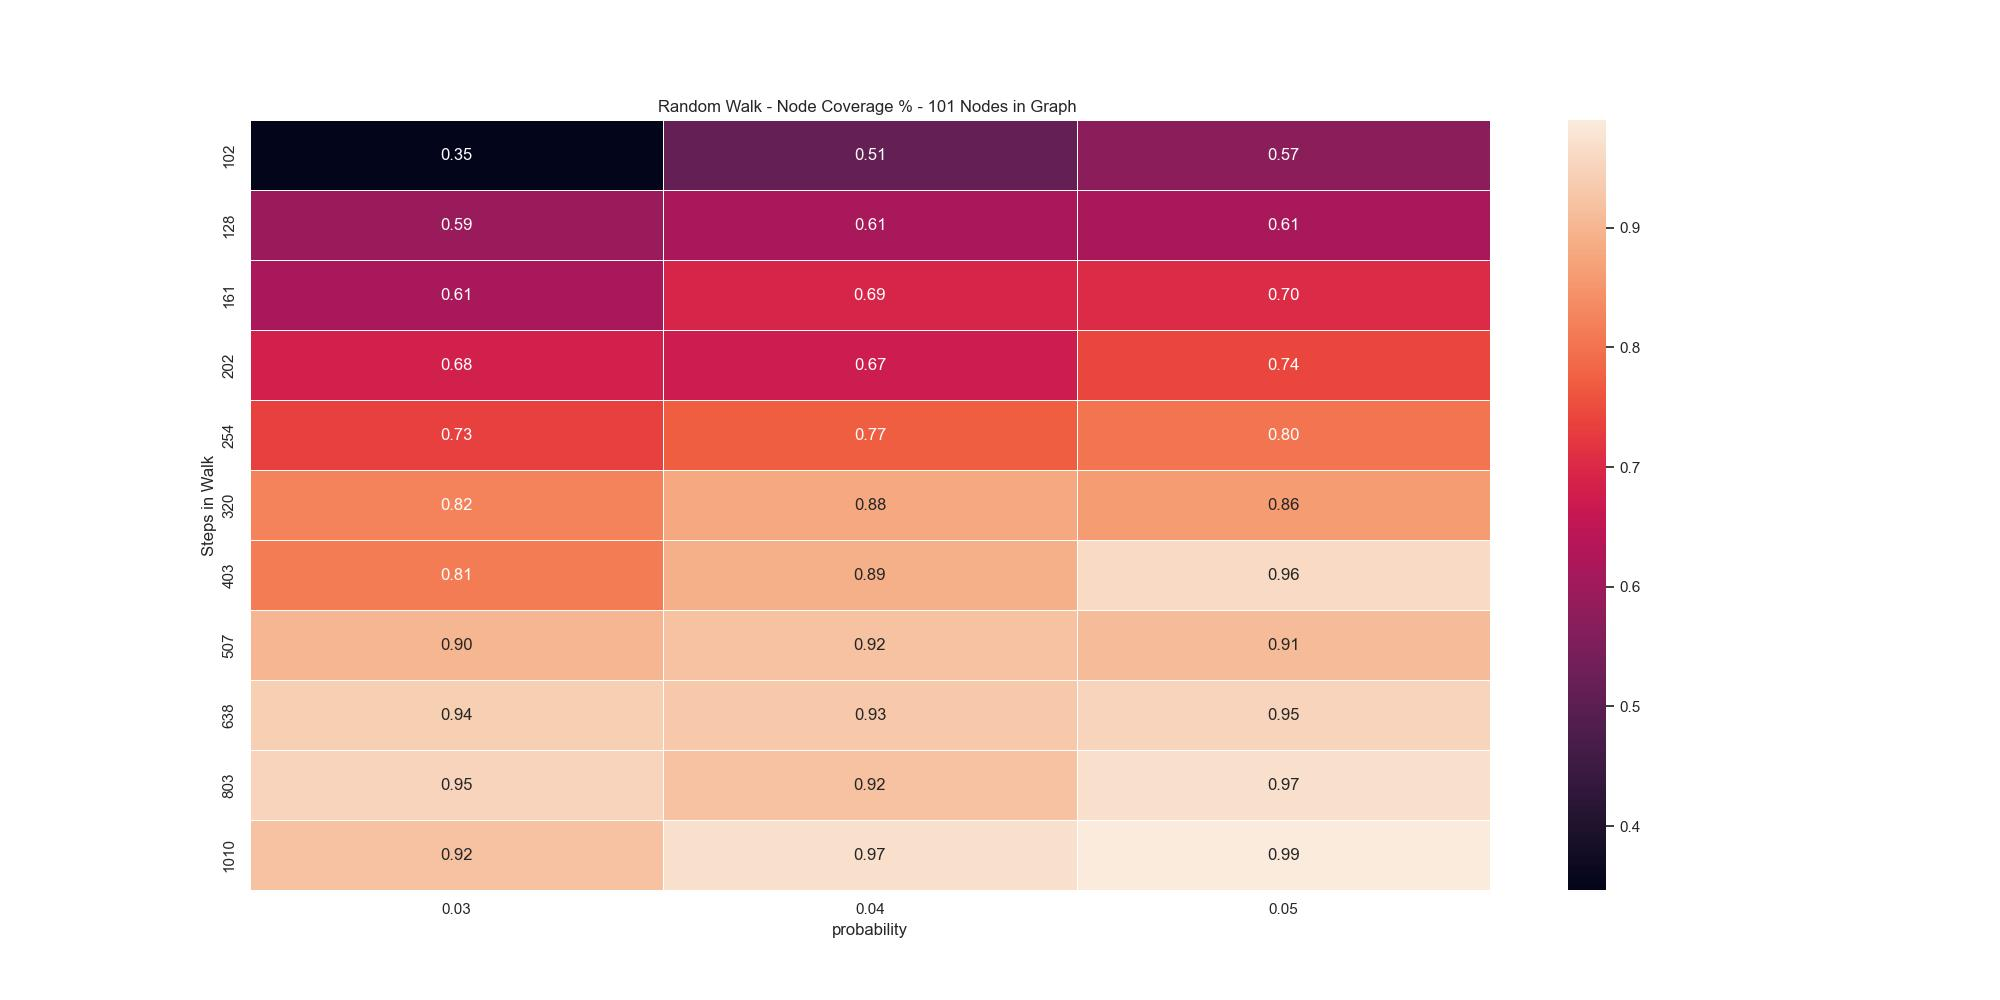
\includegraphics[width=\textwidth]{template/chapters/heatmap_lengths_unconnected_101.jpg}
    \caption{Heatmap Abdeckung in \% für n=100}
    \label{fig:cov100}
\end{figure}

\begin{figure}
    \centering
    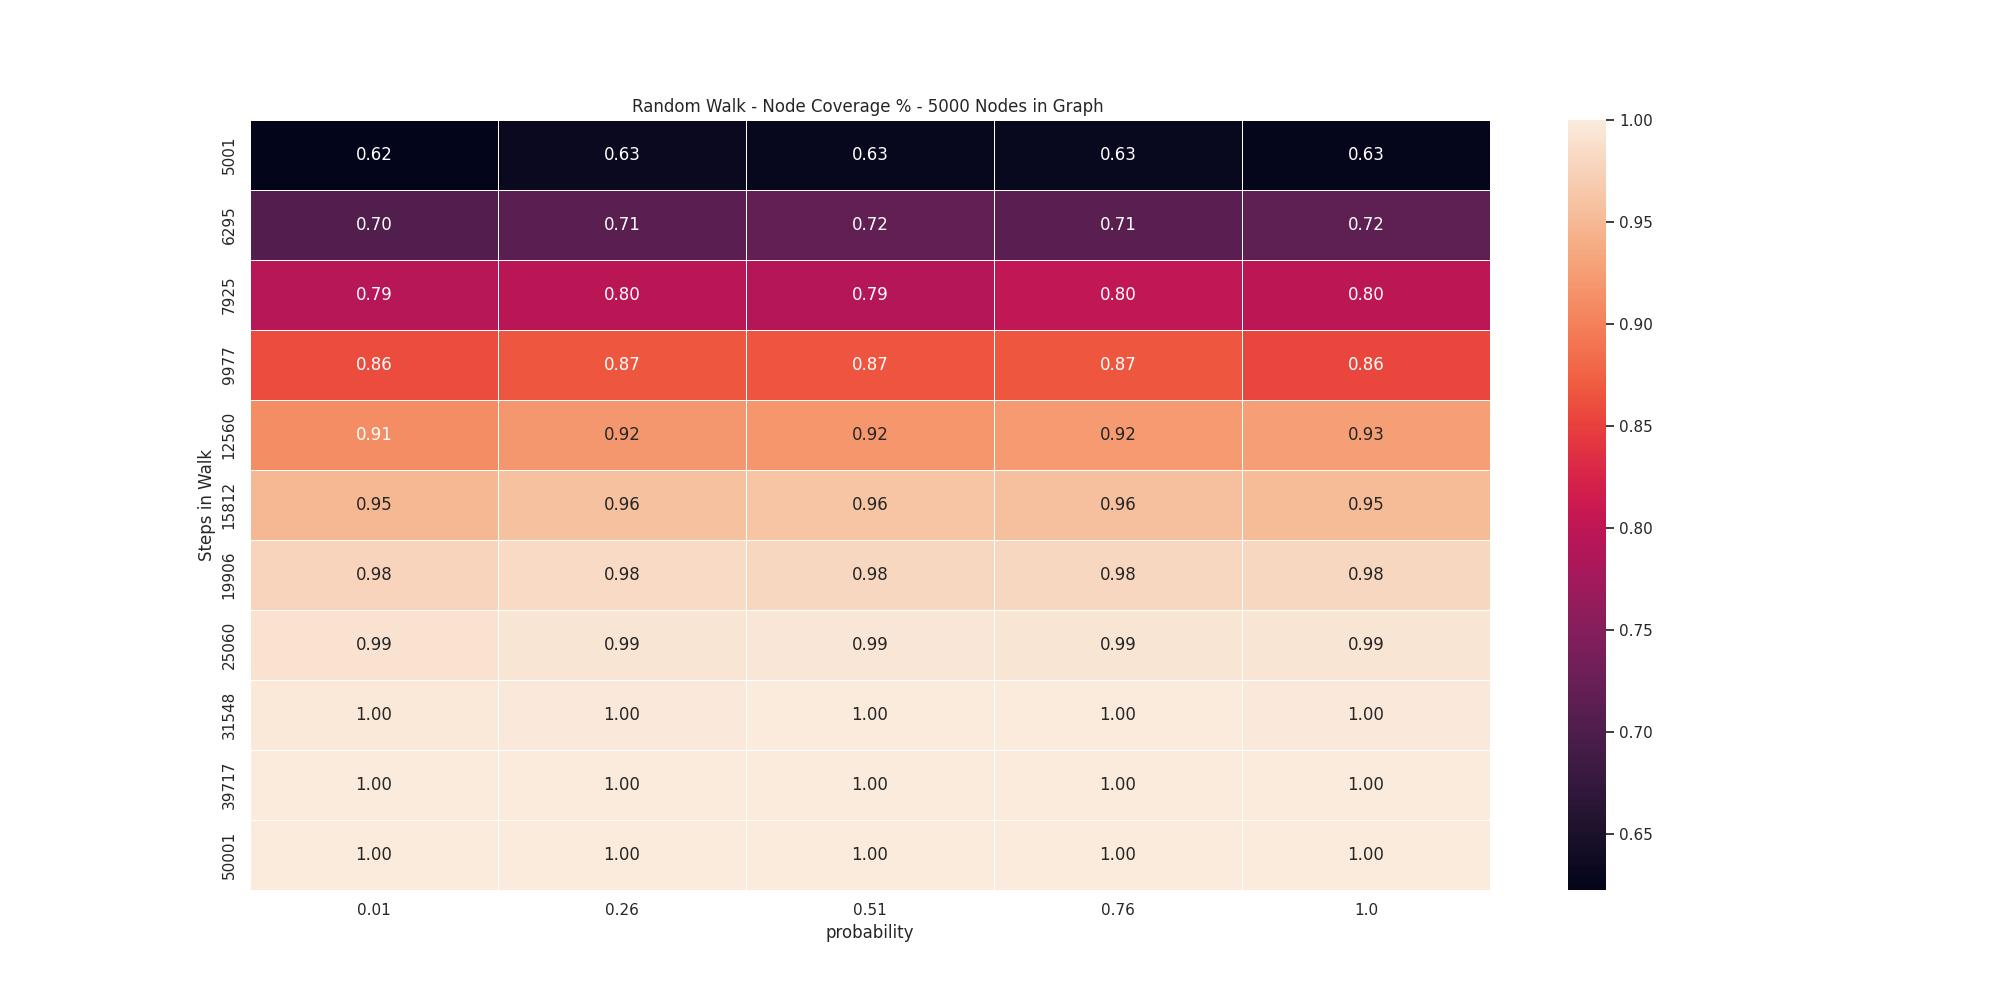
\includegraphics[width=\textwidth]{template/chapters/heatmap_lengths_unconnected_5000.jpg}
    \caption{Heatmap Abdeckung in \% für n=5000}
    \label{fig:cov5000}
\end{figure}

Beim Plotten des minimalen -Werts in Abhängigkeit von n) zeigt sich eine leichte logistische Entwicklung (die Kurve wächst zunächst schnell und verlangsamt sich später), was darauf hinweist, dass der Anstieg der benötigten Schritte nicht linear erfolgt. Dennoch kann der Wert s = n * 10 als zuverlässiger Schwellenwert verwendet werden, da er in allen getesteten Fällen stets im richtigen Bereich liegt. 

\begin{figure}
    \centering
    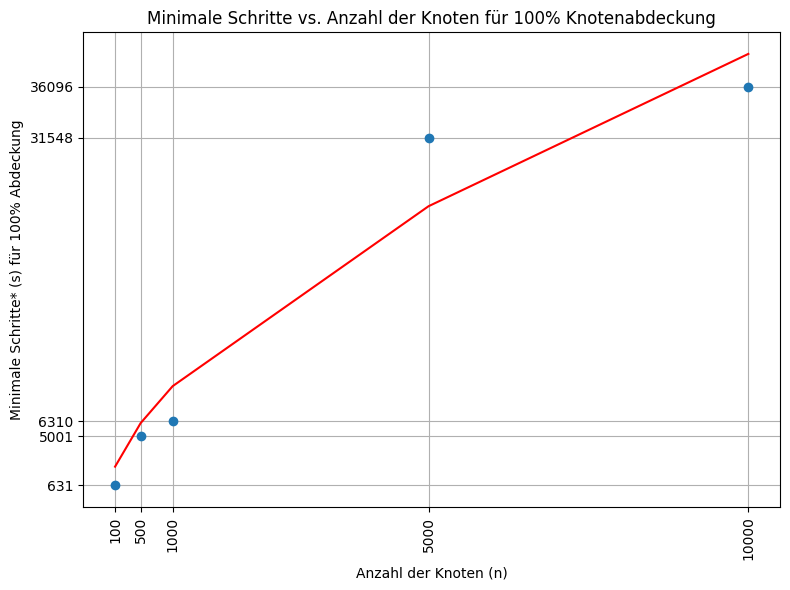
\includegraphics[width=\textwidth]{template/chapters/MinimaleSchritte-vs-AnzahlKnoten-Vollabdeckung.png}
    \caption{Verhältnis Minimale Schritte zu Anzahl der Knoten für Vollabdeckung}
    \label{fig:minsteps}
\end{figure}

Um den Schwellenwert s=n×10 weiter zu validieren, haben wir bei n=100, 500, und 1000 jeweils 10 Random Walks durchgeführt und den Mittelwert der Knotenabdeckung ermittelt. Diese Tests bestätigten, dass die Knotenabdeckung tatsächlich 100\% erreicht wird, wenn dieser -Wert verwendet wird. 

\begin{figure}
    \centering
    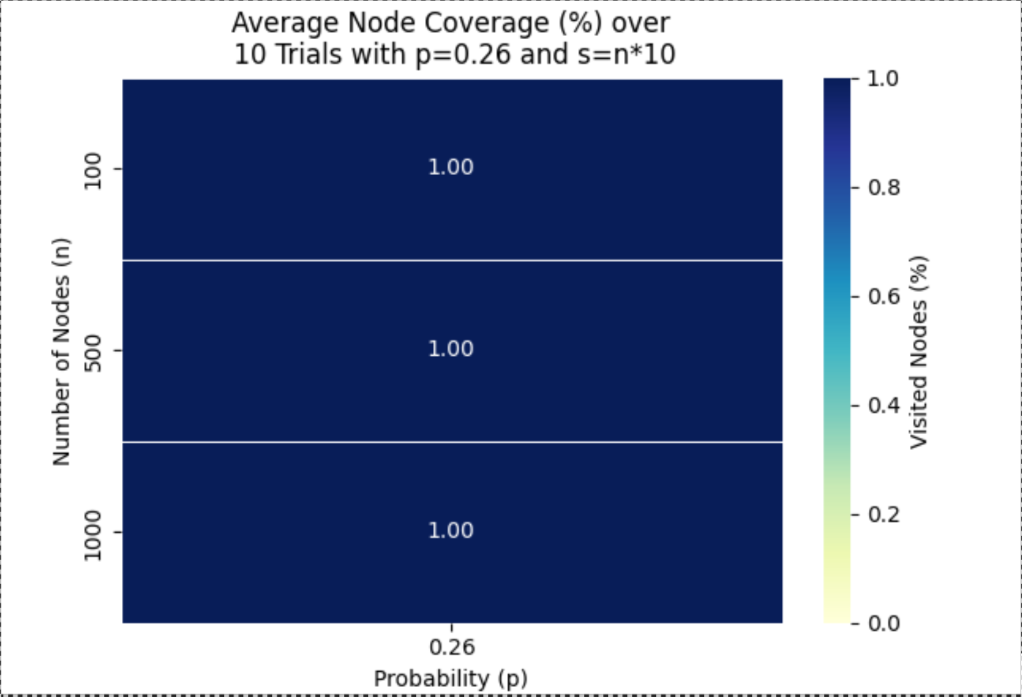
\includegraphics[width=\textwidth]{template/chapters/avg-coverage-p026-ntimes10.png}
    \caption{Mittelwert der Knotenabdeckung bei p=0.26 und s=n*10}
    \label{fig:avgcov}
\end{figure}

Schließlich haben wir in den 10 Läufen für die drei Netzwerke mit den Werten 100, 500 und 1000 die Anzahl der Besuche für die am häufigsten besuchten Knoten ermittelt. Der Modalwert der Besuche lag bei 20, 21 und 22, was zeigt, dass die Knotenabdeckung zur Analyse der Zentralitätsmaße gut geeignet ist.   

\subsection{Zentralitätsmaße}

Random Walks scheinen zu den bekannten Zentralitätsmaßen eine hohe Korrelation zu haben, siehe Abbildung \ref{fig:}
\begin{figure}
    \centering
    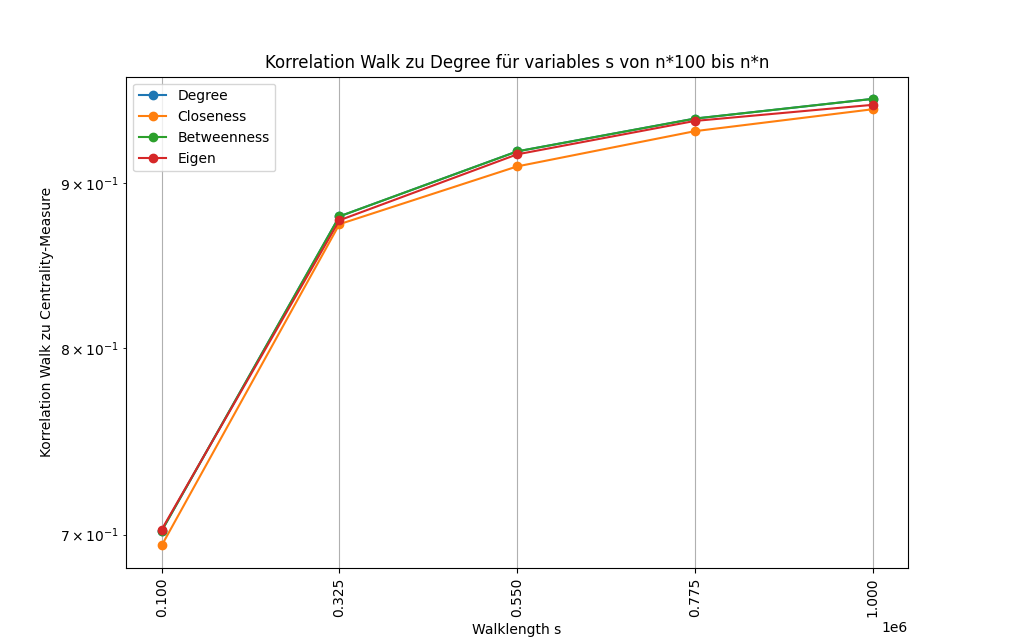
\includegraphics[width=\textwidth]{template/chapters/KorrelationWalkZuAllenAnderen_und_Eigen.png}
    \caption{Korrelation Walk zu Betweennes, Closeness, Degree, Eigen. Variables s. X-Achsen-Werte in wissenschaftlicher Notation - mal 10 hoch 6. p=0.26,n=1000}
    \label{fig:}
\end{figure} 


Hierbei führen größere s (s=n*n) zu einer sehr hohen Korrelation, siehe Abbildung \ref{fig:corr_deg_var_s}
\begin{figure}
    \centering
    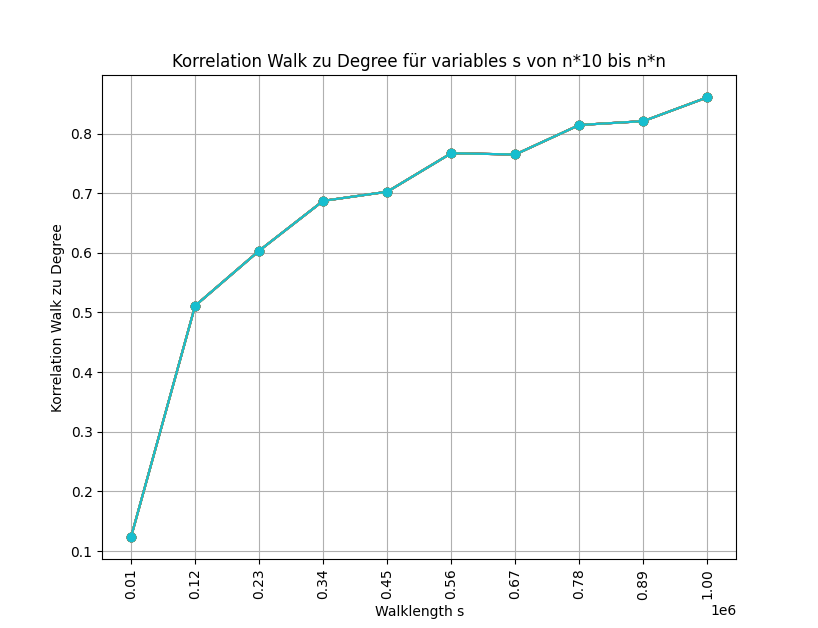
\includegraphics[width=\textwidth]{template/chapters/KorrelationWalkDegree_variables_sn10-sNtimesN.png}
    \caption{Korrelation Walk zu Degree, kleine bis sehr große s. X-Achsen-Werte in wissenschaftlicher Notation - mal 10 hoch 6. p=0.26,n=1000}
    \label{fig:corr_deg_var_s}
\end{figure}

Bei größeren n und gleichbleibender formel für s verschlechtert sich die Korrelation. Siehe Abbildung \ref{fig:corr_deg_sfix}
Dies könnte analog zu den minimale Distanzen, welche stetig Wachsen bei großem n, geschehen. 
\begin{figure}
    \centering
    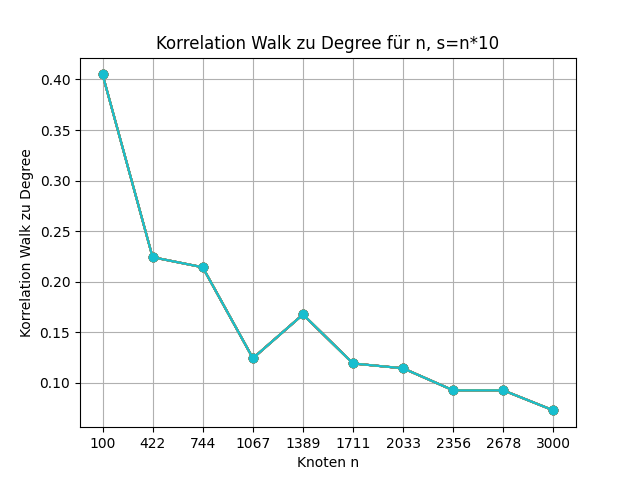
\includegraphics[width=\textwidth]{template/chapters/KorrelationWalkDegree_fixedp_sn10_v2}
    \caption{Korrelation Walk zu Degree, kleine bis sehr große n. X-Achsen-Werte in wissenschaftlicher Notation - mal 10 hoch 6. p=0.26}
    \label{fig:corr_deg_sfix}
\end{figure}


Anders als bei der Betrachtung der 100\%-Abdeckung reicht die gefundene Formeln für s in Abhängigkeit von n nicht aus für die als hoch erwartete Korrelation der Walks zu den vorgegebenen Zentralitätsmaßen
Vergleiche mit Abbildung 3  mit Abbildung %todo

%Abbildungen für obere Sachverhalte

\section{Fazit \& Ausblick}

Wir konnten eine Korrelation zwischen einem Random Walk und anderen Zentralitätsmaßen bei geeigneten Bedingungen nachweisen. 

Weitere Betrachtungen für kleinere p wären interessant, da sie natürlich vorkommenden Graphen mehr ähneln als den hier notwendigerweise sehr stark verbundenen Graphen.

%TODO


\end{document}